\documentclass[11pt,a4paper]{article}
\usepackage[utf8]{inputenc}
\usepackage[T1]{fontenc}
\usepackage{lmodern}
\usepackage{amsmath,amssymb,physics,siunitx,graphicx,booktabs,hyperref}
\usepackage[margin=2.5cm]{geometry}
\graphicspath{{figures/}}

\title{Quantum Zeeman Engine\\ \large From the normal Zeeman effect to Paschen--Back, level by level}
\author{}
\date{\today}

\begin{document}
\maketitle
\tableofcontents

\begin{abstract}
We decompose the Zeeman effect into successive levels. Each level gets a derivation (this
report), a numerical model (\texttt{src/}), a plot or animation, and a comparison with
experimental values. If the numerical result reproduces the measurement, the model underneath is
correct.
\end{abstract}

\section{Method}
For one electron with orbital momentum $l$ and spin $1/2$,
\begin{equation}
  H = H_0 + \zeta\, \vb{L}\!\cdot\!\vb{S} + \mu_B B\,(g_l L_z + g_s S_z),
\end{equation}
built as a matrix in the product basis $\ket{l,m_l}\otimes\ket{\tfrac12,m_s}$ and diagonalised
with \texttt{numpy.linalg.eigh}. The spin--orbit constant $\zeta$ is fixed from the measured
fine-structure splitting, then everything else is a prediction.

\section{Level 1: Normal Zeeman effect (orbital only)}
Ignoring spin, an electron with orbital momentum $\vb{L}$ has magnetic moment
$\vb{\mu}_l = -\mu_B \vb{L}/\hbar$, so
\begin{equation}
  H_Z = \frac{\mu_B}{\hbar} B L_z, \qquad
  \Delta E = \mu_B B\, m_l, \quad m_l = -l,\dots,l .
\end{equation}
Each level splits into $2l+1$ equally spaced components. A transition between two such
levels with $\Delta m_l = 0,\pm1$ gives three lines: the $\pi$ line (unshifted) and the two
$\sigma$ lines shifted by $\pm \mu_B B$. In wavenumbers,
$\Delta\tilde\nu = \pm \mu_B B/(hc) \approx \pm 0.4669\,B[\si{T}]\ \si{\per\centi\metre}$.
\emph{Numerical check:} set $\zeta=0$ in the code; the spectrum must be equally spaced.

\section{Level 2: Anomalous Zeeman effect (spin--orbit and Land\'e $g$)}
Spin adds a moment with $g_s \approx 2.0023$. With spin--orbit coupling
$H_{SO} = \zeta\,\vb{L}\cdot\vb{S}$ the good quantum number is $j$, with
\begin{equation}
  E_{SO}(j) = \tfrac{\zeta}{2}\big[j(j+1) - l(l+1) - s(s+1)\big],
  \qquad E(l+\tfrac12) - E(l-\tfrac12) = \zeta\,(l+\tfrac12).
\end{equation}
For weak fields ($\mu_B B \ll \zeta$) the projection theorem gives
\begin{equation}
  \Delta E = g_J\, \mu_B B\, m_j, \qquad
  g_J = 1 + (g_s - 1)\,\frac{j(j+1) + s(s+1) - l(l+1)}{2j(j+1)} .
\end{equation}
For a $p$ electron ($g_s=2$): $g_J(^2P_{1/2}) = 2/3$ and $g_J(^2P_{3/2}) = 4/3$; for $^2S_{1/2}$,
$g_J = 2$. This is why the sodium D lines split into 4 and 6 components rather than 3.
\emph{Numerical check:} \texttt{tests/test\_physical\_constants.py} verifies the slopes at small $B$.

\section{Level 3: Paschen--Back regime (strong field)}
When $\mu_B B \gg \zeta$ the Zeeman term dominates, $\vb{L}$ and $\vb{S}$ decouple, and $m_l$,
$m_s$ become good quantum numbers:
\begin{equation}
  E \simeq \mu_B B\,(m_l + g_s m_s) + \zeta\, m_l m_s .
\end{equation}
The crossover scale is $B^\ast = \zeta/\mu_B$. Levels with the same $m_j=m_l+m_s$ never cross
(they repel); levels with different $m_j$ may. The two stretched states
$\ket{m_l=\pm1, m_s=\pm\frac12}$ are exact eigenstates at every field,
$E = \zeta/2 \pm \mu_B B (1+g_s/2)$, which the tests use as an exact check.

\begin{figure}[h]
\centering
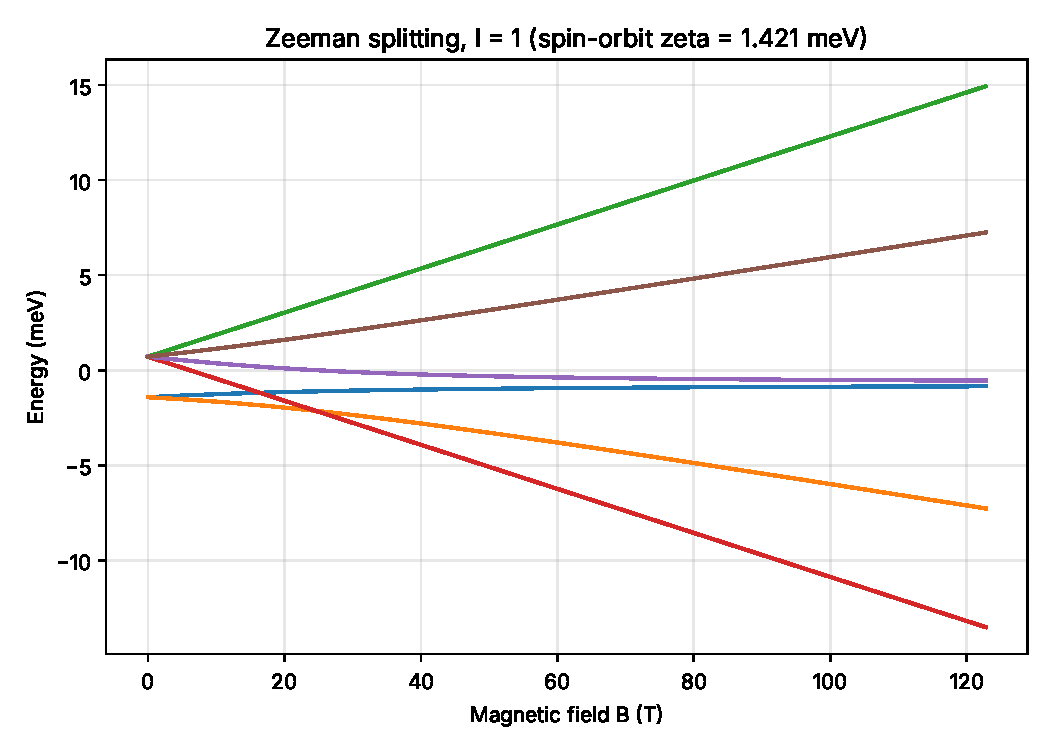
\includegraphics[width=0.8\textwidth]{p_orbital_levels.pdf}
\caption{Energy levels of a $p$ electron (sodium $3p$ spin--orbit constant) from weak field to Paschen--Back.}
\end{figure}

\section{Level 4: Wigner--Eckart theorem and spherical tensors}
\emph{Planned.} The Zeeman operator is a rank-1 spherical tensor, $H_Z \propto B\,T^{(1)}_0(\vb{L}+g_s\vb{S})$.
The Wigner--Eckart theorem factorises its matrix elements as
\begin{equation}
  \bra{\gamma' j' m'} T^{(k)}_q \ket{\gamma j m}
  = (-1)^{j'-m'}\begin{pmatrix} j' & k & j\\ -m' & q & m\end{pmatrix}
    \bra{\gamma' j'}\!\vert T^{(k)}\vert\!\ket{\gamma j},
\end{equation}
which explains the selection rules $\Delta m = 0,\pm1$ and gives intensities of the Zeeman components.
Next steps: implement the 3-$j$ symbols (\texttt{sympy.physics.wigner}), and compare relative
line intensities with experiment. The PyTorch module can then fit $\zeta$ by autograd.

\section{Extension A: Hydrogen $n=2$ and the Lamb shift}
The method of Levels 1--4 carries over to a different atom with one new idea: putting two
orbital levels, $2s$ and $2p$, into a single Hamiltonian.

\subsection{Block structure}
The eight $n=2$ states (spin included) are $2S_{1/2}$ (2 states), $2P_{1/2}$ (2) and $2P_{3/2}$ (4).
Both the spin--orbit term and the Zeeman term commute with $\vb{L}^2$, so $l$ is conserved and
\begin{equation}
  H = H(l{=}0) \oplus H(l{=}1).
\end{equation}
Energies are measured from $2P_{1/2}$ at zero field. In the $l=1$ block, $\zeta = \Delta_{2P}/(3/2)$
with $\Delta_{2P} = E(2P_{3/2}) - E(2P_{1/2})$. In the $l=0$ block, $2S_{1/2}$ is raised by the
\emph{Lamb shift} $\Delta_L = E(2S_{1/2}) - E(2P_{1/2})$. The Dirac equation predicts $\Delta_L = 0$;
it is a QED effect, so we take it from experiment ($1057.845\ \si{MHz}$).

\subsection{Consequences}
\begin{enumerate}
  \item \textbf{Weak field.} Each term moves with slope $g_J m_j$, as in Level 2
        ($g_J = 2,\ 2/3,\ 4/3$ for $2S_{1/2},\ 2P_{1/2},\ 2P_{3/2}$).
  \item \textbf{No $2s$--$2p$ mixing by $B$.} Because $l$ is conserved, levels from the two blocks
        \emph{cross} instead of repelling. Mixing them requires an electric field, the basis of the
        Lamb--Retherford experiment (not modelled here).
  \item \textbf{The crossing field measures $\Delta_L$.} The level $2S_{1/2}(m_j{=}-\tfrac12)$
        falls with slope $-g_s/2$ while $2P_{1/2}(m_j{=}+\tfrac12)$ rises with slope $+g_{1/2}/2$. A first-order estimate is
        \begin{equation}
          B_\times \approx \frac{\Delta_L}{\mu_B\,(g_s/2 + g_{1/2}/2)} = 566.5\ \si{G}.
        \end{equation}
        The exact diagonalisation gives $573.4\ \si{G}$: the field also mixes $2P_{1/2}$ with
        $2P_{3/2}$, bending $2P_{1/2}$ down by about $13\ \si{MHz}$ at this field. The literature quotes
        ``about 570 G'' (a study that also includes hyperfine structure, which our model neglects).
        Doubling $\Delta_L$ in the model moves the crossing from $573\ \si{G}$ to $1160\ \si{G}$.
\end{enumerate}

\begin{table}[h]
\centering
\begin{tabular}{lrr}
\toprule
Quantity & Reference & Model \\
\midrule
$2P_{3/2}-2P_{1/2}$ (MHz) & 10969.13 (input; Dirac theory: 10949) & input \\
$2S_{1/2}-2P_{1/2}$ Lamb shift (MHz) & 1057.845 (input) & input \\
$2S_{1/2}(-\tfrac12)\times 2P_{1/2}(+\tfrac12)$ crossing (G) & about 570 & 573.4 \\
\bottomrule
\end{tabular}
\caption{Hydrogen $n=2$. Inputs: Lamb shift $1057.845(9)$ MHz (Lundeen and Pipkin, quoted in \cite{arxiv0809}); fine structure $10969.13(10)$ MHz \cite{baird1972}.}
\end{table}

\begin{figure}[h]
\centering
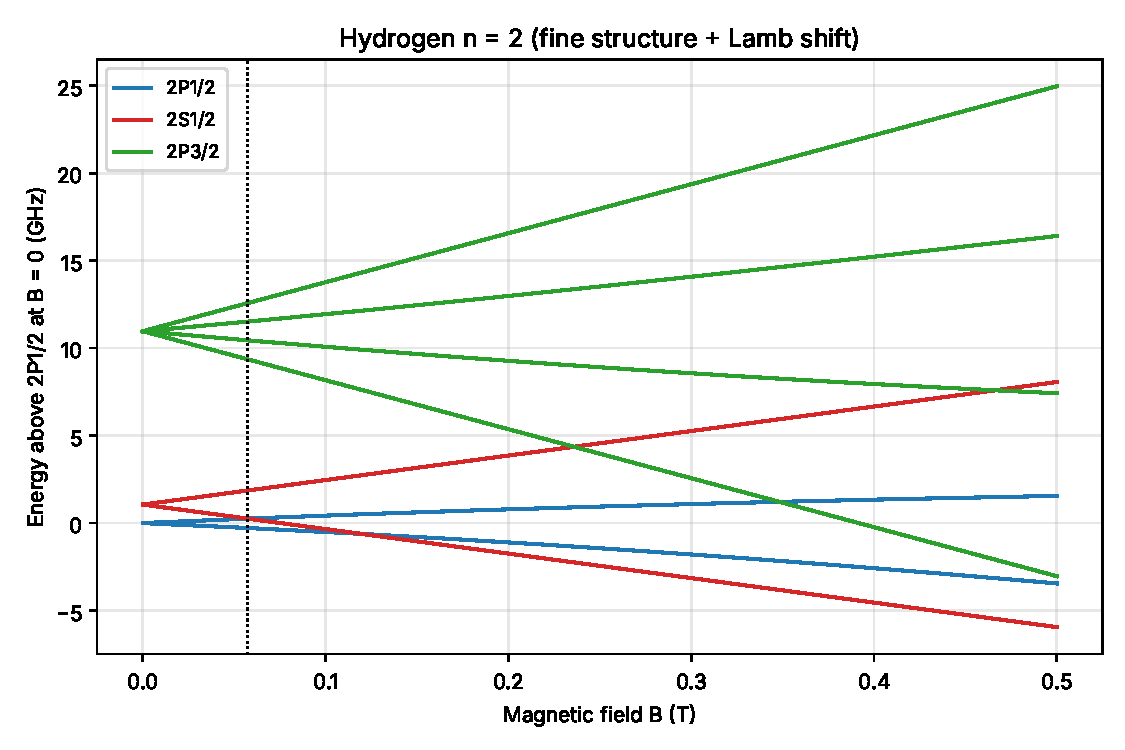
\includegraphics[width=0.8\textwidth]{hydrogen_n2_levels.pdf}
\caption{Hydrogen $n=2$ levels versus magnetic field (red: $2S_{1/2}$, blue: $2P_{1/2}$, green: $2P_{3/2}$).
The dotted line marks the crossing near 570 G.}
\end{figure}

\section{Extension B: The virtual spectrometer (colour, prism, polarisation)}
Levels 1--4 give the lines of an atom in a field. This extension puts optics in front of them:
colours, a glass prism, polarisation filters, and the question of how fine an instrument must be.
The code lives in \texttt{src/optics/}.

\subsection{Three kinds of light and two viewing directions}
With $q = m_\text{upper} - m_\text{lower}$ the atom radiates $\pi$ light ($q=0$, a dipole along $\vb{B}$)
and $\sigma^\pm$ light ($q=\pm1$, a dipole rotating around $\vb{B}$). Their angular patterns share the
same total power:
\begin{equation}
  I_\pi(\theta)\propto \sin^2\theta,\qquad
  I_{\sigma}(\theta)\propto \tfrac12\,(1+\cos^2\theta),
\end{equation}
with $\theta$ the angle between the line of sight and $\vb{B}$.
\begin{table}[h]
\centering
\begin{tabular}{lll}
\toprule
& Across $\vb{B}$ ($\theta=90^\circ$) & Along $\vb{B}$ ($\theta=0^\circ$)\\
\midrule
$\pi$ & linear, parallel to $\vb{B}$, brightness 1 & absent\\
$\sigma^\pm$ & linear, perpendicular to $\vb{B}$, brightness $\tfrac12$ & circular, opposite handedness, brightness 1\\
\bottomrule
\end{tabular}
\caption{What each viewing direction shows, for equal emission rates.}
\end{table}

\subsection{Jones calculus for the filters}
Each component has a Jones vector $\vb{J}$ (basis: along the projection of $\vb{B}$ on the sky and
perpendicular to it). With time dependence $e^{-i\omega t}$,
$\vb{J}_\pi=(-\sin\theta,\,0)$ and $\vb{J}_{\sigma^\pm}=(\cos\theta,\ \pm i)/\sqrt2$, whose squared lengths are the
patterns above. An optical element is a $2\times2$ matrix $M$ and the observed intensity of a component is
\begin{equation}
  I_\text{obs} = R\;\lvert M\,\vb{J}\rvert^2,
\end{equation}
where $R$ is the component's emission rate. A linear polariser at angle $\varphi$ gives Malus's law,
and a quarter-wave plate followed by a polariser forms a circular analyser that passes $\sigma^+$ and blocks
$\sigma^-$ (or the reverse). Different lines are incoherent, so intensities add. Which handedness is
called ``left'' or ``right'' differs between textbooks and flips if $\vb{B}$ is reversed; the code states its
convention and the tests check consistency.

\subsection{Textbook intensity ratios, reproduced}
Viewed across the field in weak field the code gives, with nothing typed in by hand:
the four D1 components are equally bright, and the D2 components have relative intensities
$4:3:1$ (the two $\pi$ lines : the inner $\sigma$ pair : the outer $\sigma$ pair).
A polariser parallel to $\vb{B}$ keeps only the $\pi$ lines, one perpendicular keeps only the $\sigma$ lines,
and along the field a circular analyser splits the $\sigma^+$ lines from the $\sigma^-$ lines.

\begin{figure}[h]
\centering
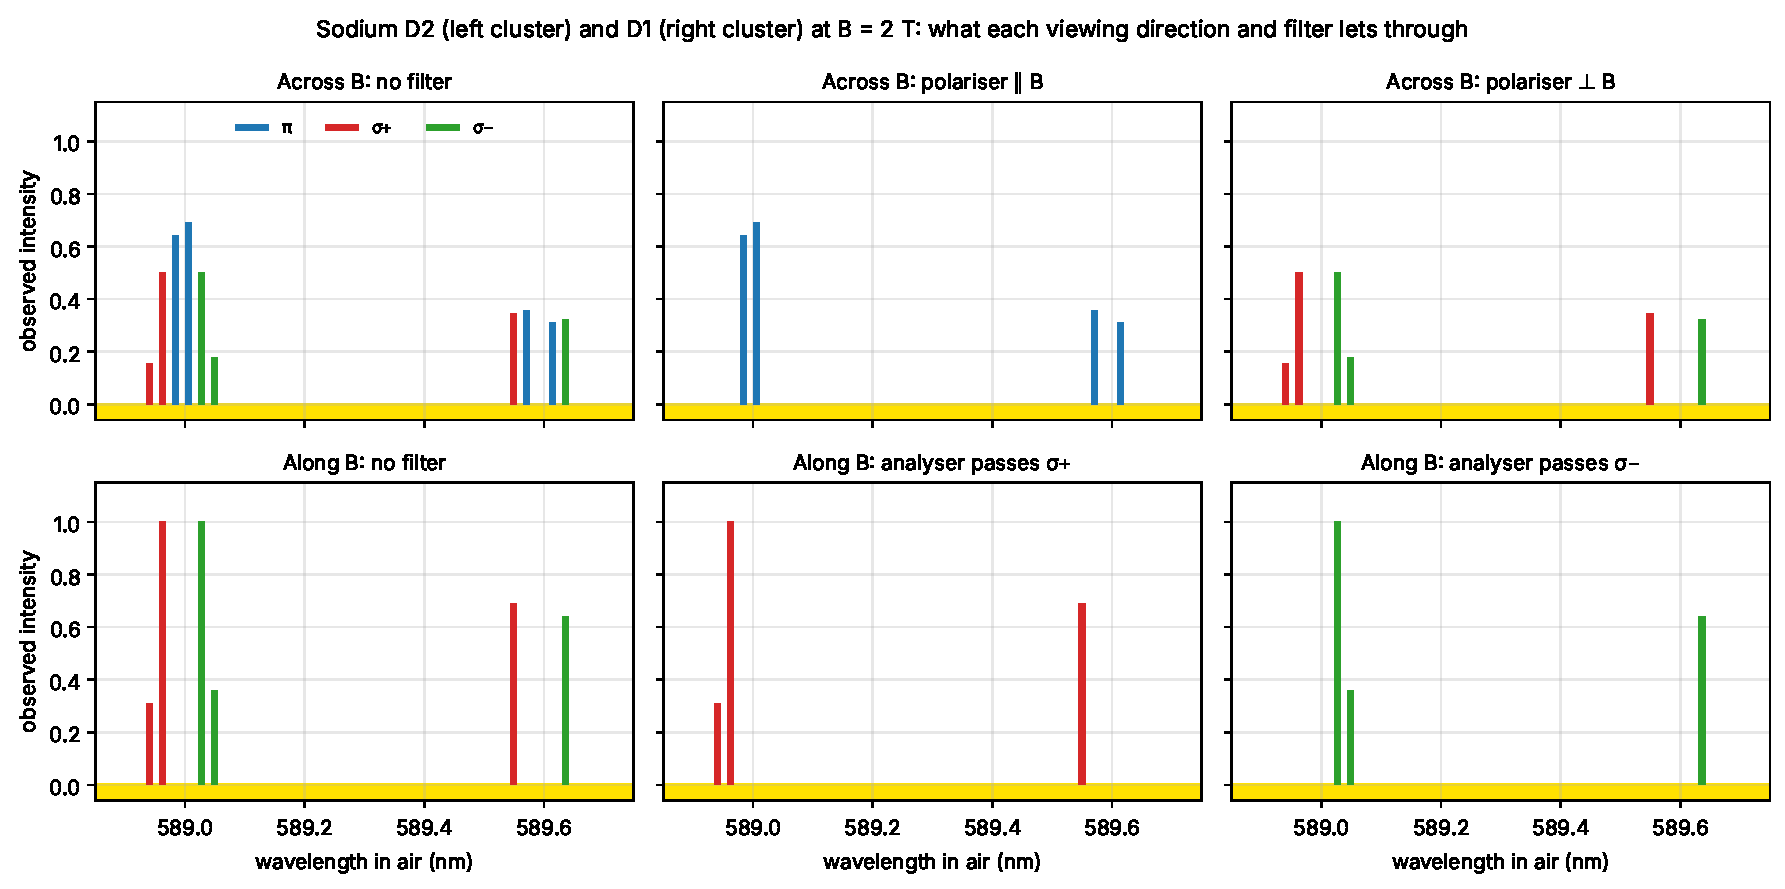
\includegraphics[width=\textwidth]{optics_polarisation_filters.pdf}
\caption{Sodium D lines at $B=2\ \si{T}$ through different filters and viewing directions.}
\end{figure}

\subsection{Colour and the prism}
A prism bends light by an amount set by $n(\lambda)$, which the code takes from the Sellmeier equation with
catalogue constants (BK7 reproduces $n_d=1.5168$). At minimum deviation
$\delta_\text{min}=2\arcsin(n\sin\tfrac A2)-A$. Violet bends most and red least, so a lamp spectrum spreads
into its colours on a screen (Figure~\ref{fig:prism}); the sodium D1 and D2 lines, only $0.6\ \si{nm}$ apart,
land close together.
\begin{figure}[h]
\centering
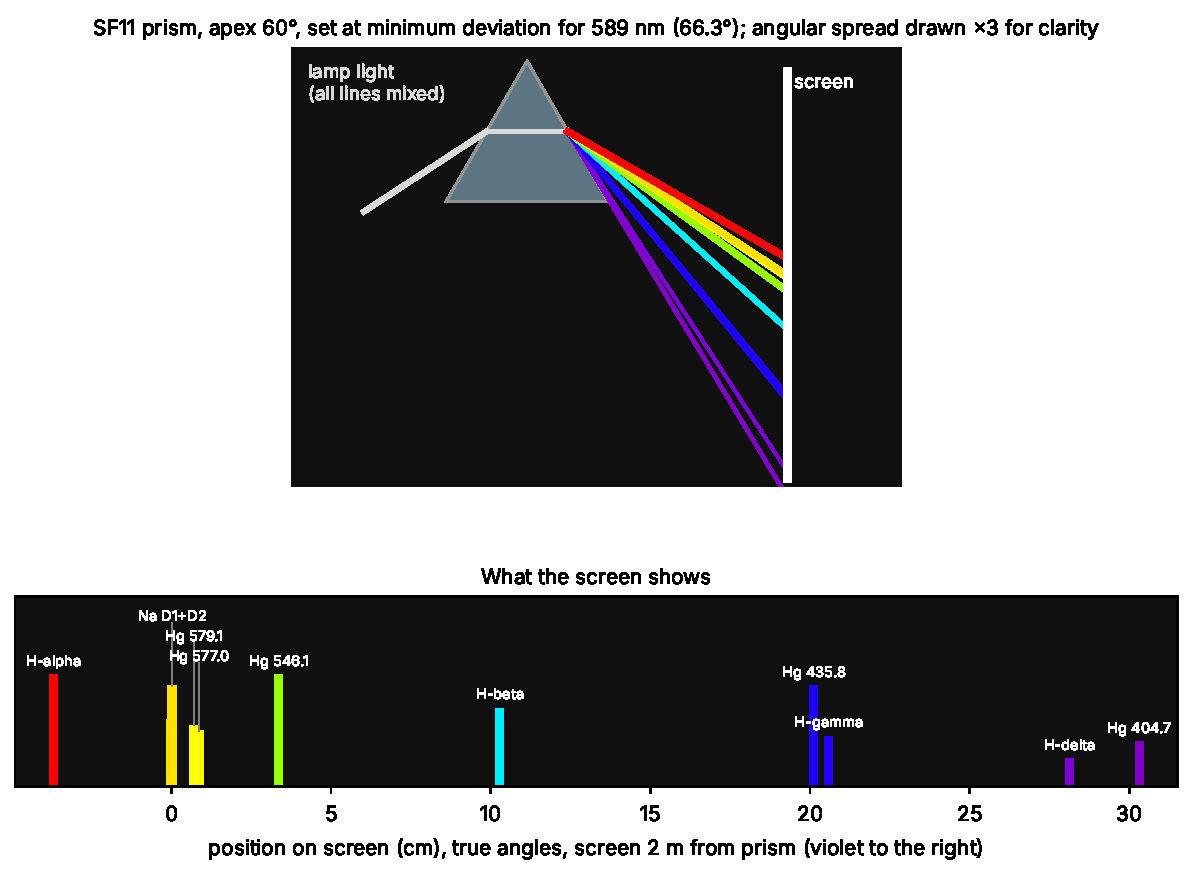
\includegraphics[width=0.85\textwidth]{optics_prism_setup.pdf}
\caption{A 60$^\circ$ SF11 prism splitting a lamp's lines (angular spread exaggerated $\times3$ in the ray drawing; the screen strip uses true angles).}
\label{fig:prism}
\end{figure}

\subsection{Can the prism show the Zeeman components?}
No. The outermost D2 component moves by only about $27\ \si{pm}$ per tesla, and all components are the same
yellow. The resolving power $R=\lambda/\Delta\lambda$ needed to separate the closest components is about
$5.5\times10^4$ at $1\ \si{T}$ and scales as $1/B$. Ideal resolving powers are about $2\times10^3$ for a 5\,cm BK7 prism,
$7.6\times10^3$ for SF11, $3\times10^4$ and $1.2\times10^5$ for gratings, and $10^6$ for a Fabry--Perot
(Figure~\ref{fig:ladder}). The weakest field at which each can just separate the components is $26$, $7.2$, $1.8$, $0.45$ and
$0.054\ \si{T}$ respectively; the BK7 prism needs about the crossover field $B^\ast=24.6\ \si{T}$, where the weak-field picture
has already ended.
\begin{figure}[h]
\centering
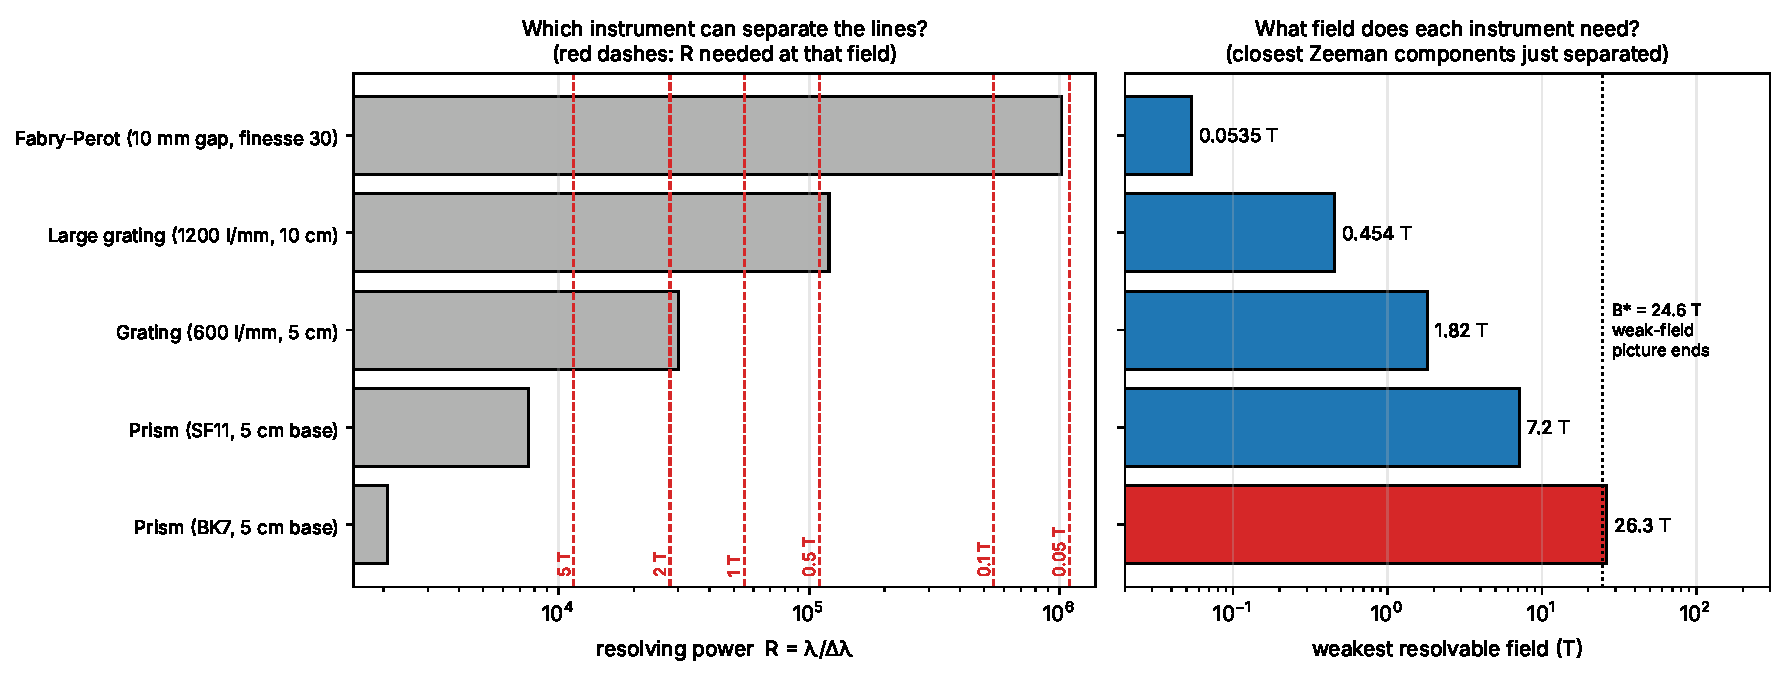
\includegraphics[width=\textwidth]{optics_instrument_ladder.pdf}
\caption{Instrument resolving powers (ideal) against the power the sodium Zeeman pattern needs.}
\label{fig:ladder}
\end{figure}


\section{Validation against experiment}
\begin{table}[h]
\centering
\begin{tabular}{lrr}
\toprule
Quantity & Reference & Model \\
\midrule
Na $3p$ fine-structure splitting (\si{\per\centi\metre}) & 17.196 & 17.196 (input) \\
$g_J(^2P_{1/2})$ & $2/3$ (0.6667) & 0.6659 ($g_s=2.0023$) \\
$g_J(^2P_{3/2})$ & $4/3$ (1.3333) & 1.3341 ($g_s=2.0023$) \\
Na D1 / D2 Zeeman components & 4 / 6 & 4 / 6 \\
Na D2\,:\,D1 intensity ratio & 2 & 2.000 \\
H $2S_{1/2}\times2P_{1/2}$ crossing (G) & about 570 & 573.4 \\
Na D2 intensities across $\vb{B}$ ($\pi$:$\sigma_\text{in}$:$\sigma_\text{out}$) & 4 : 3 : 1 & 4.00 : 2.99 : 1.00 \\
\bottomrule
\end{tabular}
\caption{Reference values are in \texttt{data/experimental\_reference.csv}. Check them against NIST ASD before publishing.}
\end{table}

\end{document}
